% !Mode:: "TeX:UTF-8:Main"
\makeatletter
\def\UlrikeFischer@package@version{0.1}
\def\UlrikeFischer@package@date{2020-03-30}
\makeatother
\RequirePackage[patches]{pdfresources}
\DeclareDocumentMetaData{pdfversion=1.7,lang=en-UK}
\documentclass[DIV=12,parskip=half-,bibliography=totoc]{scrartcl}
\usepackage{scrlayer-scrpage}
\usepackage{fontspec}
\setmainfont{Heuristica}
\usepackage{unicode-math}
\usepackage[english]{babel}
\usepackage[autostyle]{csquotes}
\usepackage{microtype}


\usepackage{listings}
\lstset{basicstyle=\ttfamily, columns=fullflexible,language=[LaTeX]TeX,
        escapechar=*,
        commentstyle=\color{green!50!black}\bfseries}
\usepackage[customdriver=hgeneric-experimental,
             pdfdisplaydoctitle=true,pdfusetitle,hyperfootnotes=false,
            ]{hyperref}
\hypupdateattribute            
\usepackage{ydoc-desc}            
\hypupdateattribute   
\usepackage{newpax}

\newpaxsetup{usefileattributes}
\title{The \pkg{newpax} package, v\csname UlrikeFischer@package@version\endcsname}
\subtitle{Reinserting annotations from included pdf file}
\date{\csname UlrikeFischer@package@date\endcsname}
\author{Ulrike Fischer\thanks{fischer@troubleshooting-tex.de}}

\begin{document}
\maketitle

\section{Introduction}

When including PDF-files in a document -- may it be with \verb+\includegraphics+ or with \verb+\includepdf+ -- clickable links and other annotations of these documents are lost.

The  \pkg{newpax} package offers some tools to reinsert these annotations. It is based in large parts
on the \pkg{pax} package from Heiko Oberdiek.

\section{Quick use instructions}
\subsection{First step: extract the annotations}
The luacode offers two functions which take as argument the name of a PDF without the extension.
The functions can be used in some lua scripts but also in some document which then must be compiled
with lualatex:

\lstinputlisting[caption=doc-extract.tex]{doc-extract.tex}

\subsection{Step two: Using the \texttt{.pax}-file with \pkg{pax.sty}}

Ensure that the \texttt{.pax} file created in the first step can be found by your main document. You can then insert your
PDF files together with their annotations like in the following listing.

\begin{itemize}
\item This works with pdflatex and lualatex. lualatex needs the extra code demonstrated in the document.
\item It needs two or three compilations until every reference is correct.
\item There is a small typo in \pkg{pax.sty} which affects clipping, the patch shown in the listing correct this.
\item Don't include PDFs with destinations twice as this will lead to duplicates.
\item If annotations should not be reinserted remove the \texttt{.pax}-file. 
\item When \pkg{hyperref} is detected you can change the color and style of link borders with hyperref options. 
\end{itemize}

\lstinputlisting[firstline=2,caption=doc-pax-test.tex]{doc-pax-test.tex}

\subsection[Alternative step two: Using the \texttt{.newpax}-file with \pkg{newpax.sty}]
{\textcolor{red}{Experimental!}: Variant of step two: Using the \texttt{.newpax}-file with \pkg{newpax.sty}}


The style \pkg{newpax} is based on \texttt{pax.sty} but extends in various way. It is an experimental package which requires the experimental pdfresources code.

\begin{enumerate}
\item clone \url{https://github.com/latex3/pdfresources}
\item In the main folder run \lstinline+ l3build install +. This will install the package in your texmfhome.
\end{enumerate}

\textbf{Attention!} \textcolor{red}{Experimental} means EXPERIMENTAL! The code is currently in full flow. And it is \emph{not} yet compatible with every other package.

The following listing shows how to use \pkg{newpax.sty}.

\begin{itemize}
\item It should work with pdflatex, lualatex and xelatex. (latex and dvips fails as this can't include PDF anyway).
\item Some provision have been added to allow multiple inclusion of the same PDF, but if you insert different sets of pages of a PDF destinations can be missing. So better avoid it. 
\item You can choose for every file if border color and styles of links are taken from the source PDF or from the hyperref settings. But you can't adjust or change colored links. 
\end{itemize}


\lstinputlisting[firstline=2,caption=doc-newpax-test.tex]{doc-newpax-test.tex}

\subsection{Combining the steps}

When using lualatex the code to write the pax/newpax-files can be in the main document. 

In the future it would be nice if the luacode could like e.g. epstopdf be called on the fly by a document. 

\section{Background}

Clickable links in a PDF are one example of an annotation. Annotations are areas on a page which are associated with an action. A typical annotation object could look like this in the PDF:

\begin{lstlisting}
15 0 obj
<<
/Type /Annot
/Subtype/Link
/Rect [147.716 654.025 301.887 665.15]
/Border[0 0 1]/BS<</S/U/W 1>>/H/I/C[0 1 1]
/A<</Type/Action/S/URI/URI(https://www.latex-project.org)>>
>>
endobj
\end{lstlisting}
This is an object of type \texttt{Annot} and subtype \texttt{Link}.
The \texttt{/Rect} value describes the rectangle of this annotation.  The coordinates are absolute coordinates related to the current page. It is important to understand that an annotation is not connected to some page content!
The \texttt{/Border} setting and the other values on this line describe the look and color of annotation. The \texttt{/A} value contains the action, in this case it is an url to an external website.


To \enquote{reactivate} the annotations of an included pdf one has to do a number of tasks.
\begin{itemize}
\item One must \emph{retrieve and store} the annotations of the included pdf. For links to external links this requires to find only one object like the one shown above. But e.g. internal links point to a destination object and these must be found too.
\item One must \emph{recalculate} the rectangle coordinates to fit to the coordinate system of the target page: as the included pdf can be placed at various positions, scaled, rotated and even clipped this is not an easy task. Destinations have rectangles too that must be recalculated.
\item  One must  \emph{reinsert} the annotation and related objects. This has to take into account the a pdf is perhaps not included completly, a link shouldn't point to a missing page or a clipped annotation. It also has to take into account that a pdf is perhaps inserted more than once or in steps.
\end{itemize}

\subsection{Retrieving and storing annotations}

Theoretically one can do it manually: Uncompress the PDF (or when using \LaTeX, create directly an uncompressed one), open it in an editor and copy and paste all needed objects. Practically one naturally want some tool.

The \pkg{pax} package from Heiko Oberdiek consists of a perl script and a java-jar file \texttt{PDFAnnotExtractor} which can extract the necessary objects. It writes the information to a file with the extension \texttt{pax}.
When it has been successfully install it works quite fine. Problems with this approach are
\begin{itemize}
\item \texttt{PDFAnnotExtractor} requires an external, old version of the java library of PDFbox which must be installed manually.
\item It requires a java installation and
\item it is not extensible.
\end{itemize}

The \pkg{newpax} package comes with a lua-file. It uses the \texttt{pdfe} library embedded in luatex to extract the annotations and other needed information. \pkg{newpax} writes the information to a file with the extension \texttt{pax} or \texttt{newpax}. The content of the files is (nearly) identical to the content of the \texttt{pax}-file written by \texttt{PDFAnnotExtractor}. The lua code was written by looking at example outputs from \texttt{PDFAnnotExtractor} and reproducing it in lua. The ordering of element is a bit different and some strings are output in a different way but for the examples I used the resulting \texttt{pax}-files can be used together with the original \texttt{pax.sty}. It is possible that the lua code is not yet handling all objects or options that \texttt{PDFAnnotExtractor} outputs, but the code can rather easily be extended later.


\section{Importing annotations with the \pkg{pax} package}

The \pkg{pax} package from Heiko Oberdiek does the hard work to recalculate the annotation rectangles and to decide which annotation and which destination should be reinserted. It also patches the \verb+\includegraphics+ command to automate this. 

\pkg{newpax} reuses the core commands of \pkg{pax}. It adds a number of switches and changed primitive so that more engines and backend can be supported.


\section{Example}

\fbox{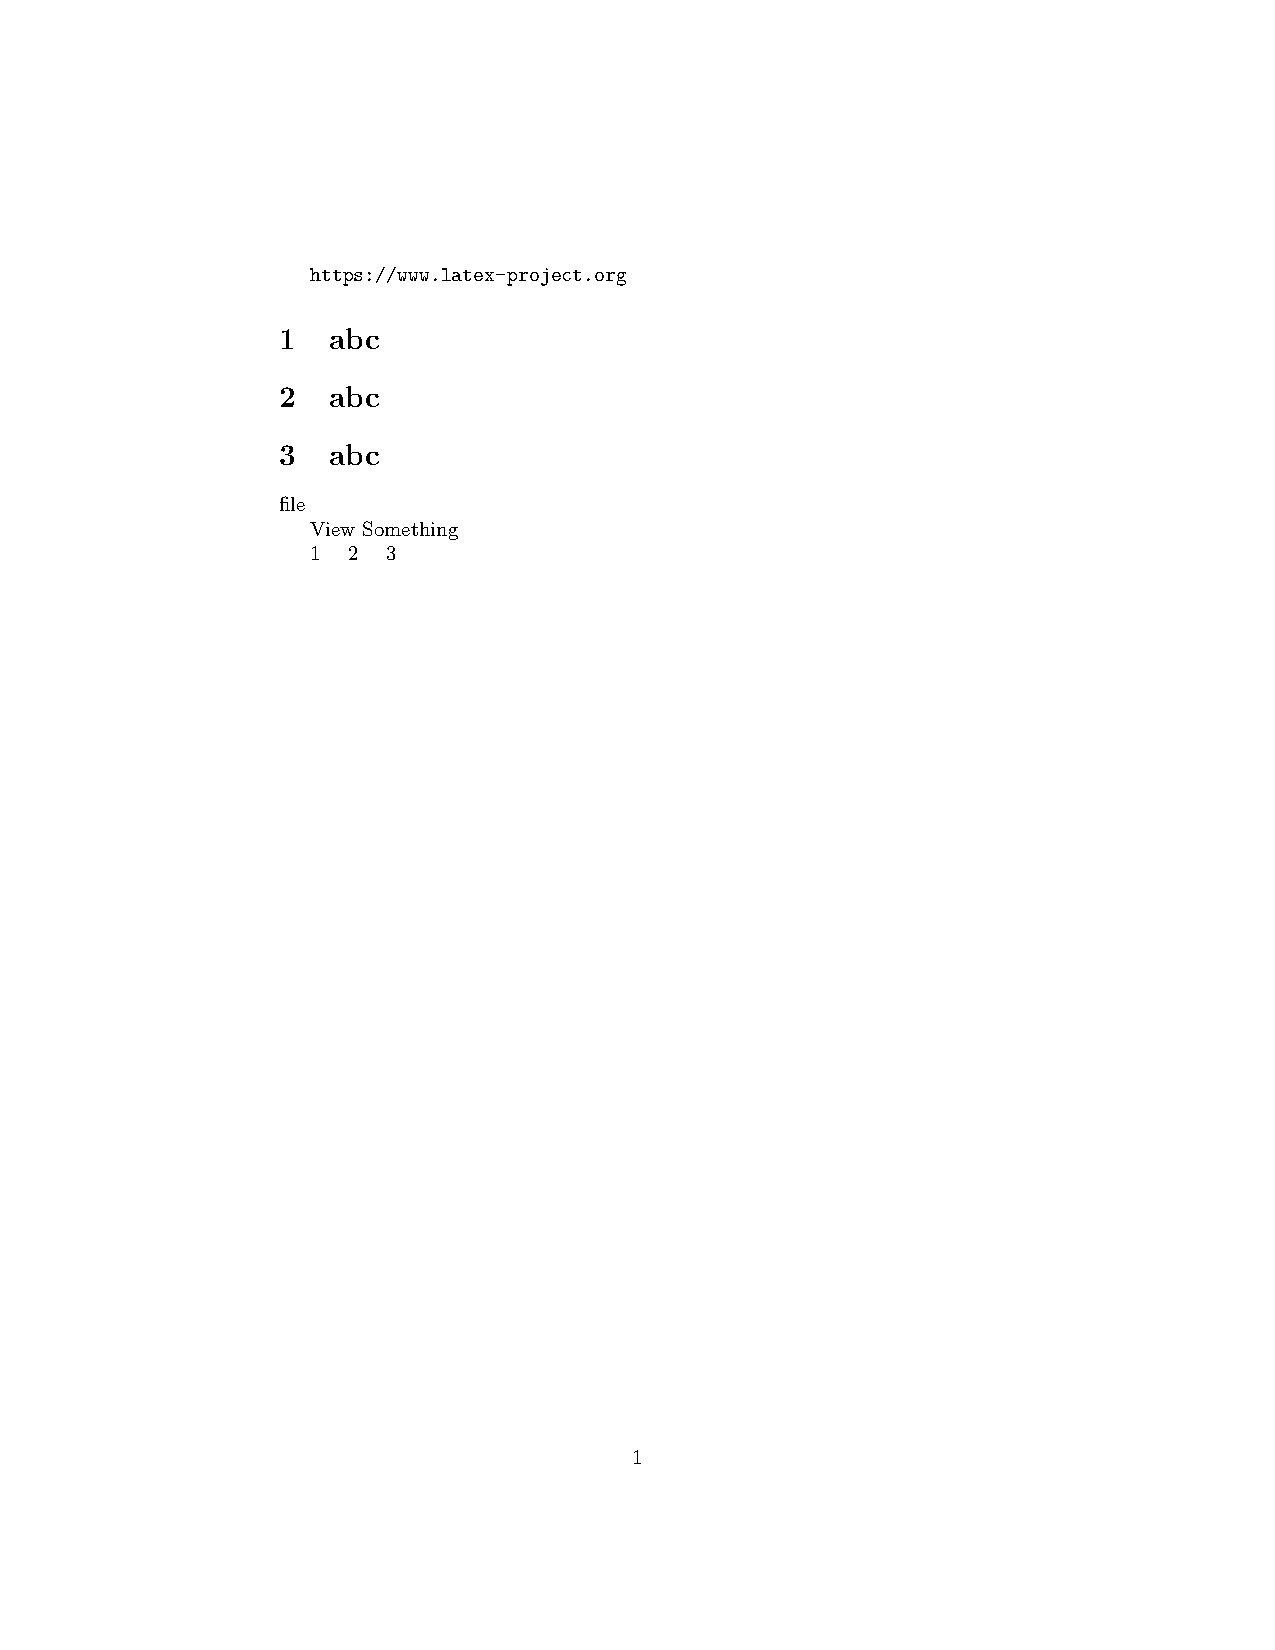
\includegraphics[scale=0.5,trim=4cm 15cm 8cm 3cm,clip,page=1]{pax-input}}
\fbox{\includegraphics[scale=0.5,trim=5cm 15cm 8cm 3cm,clip,page=2]{pax-input}}
\end{document}
